\documentclass[9pt]{article}

\usepackage{amsmath}
\usepackage{tcolorbox}
% `parskip` removes indentation for all paragraphs: http://tex.stackexchange.com/a/55016
\usepackage{parskip}
% Allows us to color rows / cols of a table.
% See https://texblog.org/2011/04/19/highlight-table-rowscolumns-with-color/
\usepackage{color, colortbl}

\usepackage{hyperref}
\graphicspath{{images/ps5/}}

\leftmargin=0.25in
\oddsidemargin=0.25in
\textwidth=6.0in
\topmargin=-0.25in
\textheight=9.25in

\definecolor{Gray}{gray}{0.9}

\begin{document}

\begin{center}
  \large\textbf{MIT 18.01 Problem Set 5 Unofficial Solutions}
\end{center}

\begin{tcolorbox}
  \textbf{Q1a)} Suppose that at the beginning of day 0, some time last summer, the temperature in Boston was $y(0) = 65^{\circ}$ Fahrenheit and that over a 50-day period, the temperature increased according to the rule $y'(t) = y(t) / 100$, with time $t$ measured in days. Find the formula for $y$, and draw a graph of temperature on days 3 and 4, $3 <= t <= 5$, and label with the correct day and shade in the regions whose areas represent the average temperature each of the two days.\footnote{The continuous average of a function is $\frac{1}{b - 1} \int_{a}^{b} f(x) dx $ . In this case $b - a = 1$, so the average is the same as the integral. For more, see Notes, AV and Lecture 23.}
\end{tcolorbox}

Based on the rule given, we calculate the temperatures from $t = 0$ to $t = 5$:

\begin{center}
  \begin{tabular}{|c|c|}
    \hline
    \rowcolor{Gray}
    $t$ & $y(t)$ \\ \hline
    0 & 65 \\ \hline
    1 & 65 + 65 / 100 = 65.65 \\ \hline
    2 & 65.65 + 65.65 / 100 = 66.3065 \\ \hline
    3 & 66.3065 + 66.3065 / 100 = 66.969565 \\ \hline
    4 & 66.969565 + 66.969565 / 100 = 67.63926065 \\ \hline
    5 & 67.63926065 + 67.63926065 / 100 = 68.3156532565 \\ \hline
  \end{tabular}
\end{center}

From the formula $y'(t) = y(t) / 100$, we get $\frac{dy}{dt} = \frac{y}{100}$. Then

\begin{align*}
  \frac{dy}{dt} &= \frac{y}{100} \\
  \frac{1}{y} dy &= \frac{1}{100} dt \\
  ln(|y|) &= \frac{1}{100} t + C \\
\end{align*}

Since $y > 0$ and is increasing,

\begin{align*}
  ln(y) &= \frac{1}{100}t + C \\
  y &= e^{\frac{1}{100}t + C} \\
  &= e^{C} \cdot e^{\frac{1}{100}t} \\
  &= Ae^{\frac{1}{100}t}
\end{align*}

At $t = 0, y = 65$. Hence $65 = Ae^{\frac{1}{100} \cdot 0} = A$. Then $ln(y) = 65e^{\frac{1}{100}t}$ \\

Graph:

\begin{center}
  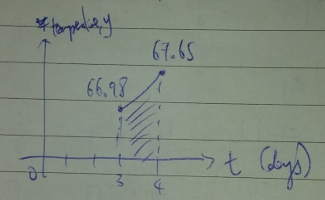
\includegraphics{q1a.jpg}
\end{center}

\begin{tcolorbox}
  \textbf{Q1b)} The number of \emph{cooling degree days} is the sum of reach day of the difference between the average temeperature for that day and $65^{\circ}$. The number is used to estimate the demand for electricity for air conditioning. Draw a second graph of $y$ for the whole 50 days and shade in the region whose area represents the total number of degree days. Write a formula for this total area as the difference between $65 \cdot 50$ and a definite integral. Evaluate the definite integral using the fundamental theorem of calculus. (Alternatively, write the whole quantity as an integral expressing the area between curves as in Lecture 21, and 7.2.)
\end{tcolorbox}

\begin{center}
  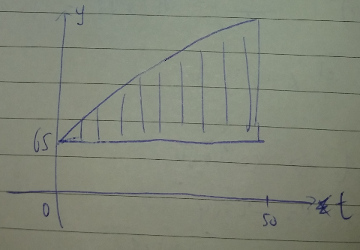
\includegraphics{q1b.jpg}
\end{center}

\begin{align*}
  A &= \int_0^{50} 65 e^{\frac{1}{100}t} dt - 65 \cdot 50 \\
  &= 6500e^{\frac{1}{100}t}\bigg]_0^{50} - 65 \cdot 50 \\
  &= 6500 (e^{\frac{50}{100}} - e^{0}) - \frac{1}{2} \cdot 6500 \\
  &= 6500 (e^{\frac{1}{2}} - \frac{3}{2}) \\
  &\approx 966.688
\end{align*}


\begin{tcolorbox}
  \textbf{Q1c)} (extra credit) Compute the definite integral in part (b) directly by evaluating a lower Riemann sum and taking a limit. Follow the procedure in Problem 5, PS4, but with different scale factors. This rather elaborate calculation shows how much time and effort we save every time we use the fundamental theorem and the change of variable formula in integrals.
\end{tcolorbox}

\begin{center}
  $\int_0^{50} 65 e^{\frac{1}{100}t} dt = 65 \int_0^{50} e^{\frac{1}{100}t} dt$
\end{center}

Since $\frac{d}{dt} e^{\frac{1}{100}t} = \frac{1}{100} e^{\frac{1}{100}t} > 0$, $e^{\frac{1}{100}t}$ is an increasing function. Hence the left Riemann sum is the lower Riemann sum.

Left Riemann sum of $\int_0^{50} e^{\frac{1}{100}t} dt = \sum\limits_{i=0}^{n-1} e^{\frac{1}{100}t_i} \Delta t$ where $\Delta t = \frac{50 - 0}{n} = \frac{50}{n}$

\begin{align*}
  \sum\limits_{i=0}^{n-1} e^{\frac{1}{100}(\frac{50i}{n})} \cdot \frac{50}{n} &= \frac{50}{n} \sum\limits_{i=0}^{n-1} e^{\frac{50i}{100n}} \\
  &= \frac{50}{n} \sum\limits_{i=0}^{n-1} e^{\frac{i}{2n}} \\
  &= \frac{50}{n} \cdot \frac{1(1 - (e^{\frac{1}{2n}})^n)}{1 - e^{\frac{1}{2n}}} \\
  &= \frac{50}{n} \cdot \frac{1 - e^{\frac{1}{2}}}{1 - e ^{\frac{1}{2n}}}
\end{align*}

Use linear approximation for $1 - e^{\frac{1}{2n}}$.

The linear approximation for $e^x = 1 + x$ for $x \approx 0$. Since $\frac{1}{2n} \rightarrow 0$ as $n \rightarrow +\infty$, then $1 - e^{\frac{1}{2n}} \approx 1 - (1 + \frac{1}{2n}) = -\frac{1}{2n}$

Then $n(1 - e^{\frac{1}{2n}}) \approx n \cdot (- \frac{1}{2n}) \approx -\frac{1}{2}$. As $n \rightarrow +\infty$,

\begin{align*}
  \sum\limits_{i=0}^{n-1} e^{\frac{1}{100}(\frac{50i}{n})} \cdot \frac{50}{n} &\approx \lim_{n \rightarrow +\infty} \frac{50}{n} \cdot \frac{1 - e^{\frac{1}{2}}}{1 - e ^{\frac{1}{2n}}} \\
  &\approx \lim_{n \rightarrow +\infty} \frac{50 \cdot (1 - e^{\frac{1}{2}})}{-\frac{1}{2}} \\
  &= -100(1 - e^{\frac{1}{2}}) \\
  &= 100e^{\frac{1}{2}} - 100
\end{align*}

Thus $\int_0^{50} e^{\frac{1}{100}t} dt \approx 100e^{\frac{1}{2}} - 100$ and $65 \int_0^{50} e^{\frac{1}{100}t} dt \approx 65(100e^{\frac{1}{2}} - 100) = 6500e^{\frac{1}{2}} - 6500$


\begin{tcolorbox}
  \textbf{Q2} Consider the function $f(x) = \int_0^{x} cos(t^2) dt$. There is no expression for $f(x)$ in terms of standard elementary functions. It is known as a Fresnel integral, along with the corresponding sine integral. \\
  a) Draw a rough sketch of $cos(t^2)$, showing the first positive and negative zeros. What does the curve look like at $t = 0$? Is the function even or odd?
\end{tcolorbox}

\begin{center}
  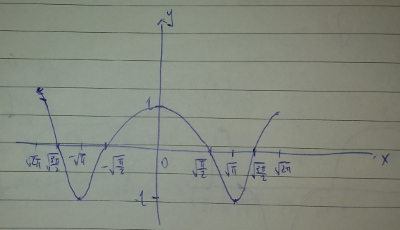
\includegraphics{q2a.jpg}
\end{center}

It is an even function.

\begin{tcolorbox}
  \textbf{Q2b)} List the critical points of $f(x)$ in the entire range $-\infty < x < \infty$. Which critical points are local maxima and which ones are local minima?
\end{tcolorbox}

$\frac{d}{dx}cos(x^2) = 2x(-sin(x^2)) = -2x\ sin(x^2)$

At critical points, $-2x\ sin(x^2) = 0$. Either $x = 0$ or $sin(x^2) = 0$ which implies $x^2 = n\pi$ for some integer $n >= 0$, which means $x = \pm\sqrt{n\pi}$ for some integer $n >= 0$

$\frac{d}{dx}-2x\ sin(x^2) = -2sin(x^2) - 4x^2cos(x^2)$

At $x = 0$, $-2sin(x^2) = 4x^2cos(x^2)$. Either $x = 0$ or $-\frac{1}{2}tan(x^2) = x^2$.

At $x = \pm\sqrt{n\pi}$ for odd $n > 0$, $-4(\pm\sqrt{n\pi})^2cos((\pm\sqrt{n\pi})^2) = -4n\pi cos(n\pi) = -4n\pi (-1) = 4n\pi > 0$. So minimum points are at $\pm\sqrt{n\pi}$ for odd $n > 0$.

At $x = \pm\sqrt{n\pi}$ for even $n$, $-4(\pm\sqrt{n\pi})^2cos((\pm\sqrt{n\pi})^2) = -4n\pi cos(n\pi) = -4n \pi < 0$. So maximum points are at $x = \pm\sqrt{n\pi}$ for even $n > 0$.

When $-4x^2cos(x^2) = 0$, either $x^2 = 0 (x = 0)$ or $cos(x^2) = 0$, which implies $x^2 = \frac{\pi}{2} + n\pi$ for any integer $n >= 0$. That is $\frac{\pi + 2n\pi}{2} = \pi(\frac{2n + 1}{2})$. Hence $x = \pm\sqrt{\pi(\frac{2n + 1}{2})}$ for any integer $n >= 0$.

In summary:

$x = \pm\sqrt{n\pi}$ for odd integer $n > 0$ are minimum points. \\
$x = \pm\sqrt{n\pi}$ for even integer $n > 0$ are maximum points. \\
$x = 0$ is inflection point. \\
$x = \pm\sqrt{\pi(\frac{2n+1}{2})}$ for any integer $n >= 0$ are inflection points.


\begin{tcolorbox}
  \textbf{Q2c)} Sketch the graph of $f$ on the interval $-2 <= x <= 2$, with labels for the critical points \textbf{and inflection points}. (The drawing should be qualitatively correct, but just estimate the values of $f$ at the labelled points.)
\end{tcolorbox}

Skipped.


\begin{tcolorbox}
  \textbf{Q2d)} Estimate $f(0.1)$ to six decimal places.
\end{tcolorbox}

$f(0.1) = \int_0^{0.1} cos(t^2) dt$

Compute fourth derivative of $cos(t^2)$

\begin{align*}
  \frac{d}{dt}cos(t^2) &= 2t(-sin(t^2)) = -2tsin(t^2) \\
  \frac{d^2}{dt^2}cos(t^2) &= \frac{d}{dt}(-2tsin(t^2)) \\
  &= -2sin(t^2) - 2t(2tcos(t^2)) \\
  &= -2sin(t^2) - 4t^2cos(t^2) \\
  \frac{d^3}{dt^3}cos(t^2) &= \frac{d}{dt}(-2sin(t^2) - 4t^2cos(t^2)) \\
  &= -2(2t)cos(t^2) - 8tcos(t^2) - 4t^2(2t \cdot (-sin(t^2))) \\
  &= -4tcos(t^2) - 8tcos(t^2) + 8t^3sin(t^2) \\
  &= -12tcos(t^2) + 8t^3sin(t^2) \\
  \frac{d^4}{dt^4}cos(t^2) &= \frac{d}{dt}(-12tcos(t^2) + 8t^3sin(t^2)) \\
  &= -12cos(t^2) - 12t(2t \cdot (-sin(t^2))) + 24t^2 sin(t^2) + 8t^3 \cdot 2tcos(t^2) \\
  &= -12cos(t^2) + 24t^2sin(t^2) + 24t^2sin(t^2) + 16t^4cos(t^2) \\
  &= -12cos(t^2) + 48t^2sin(t^2) + 16t^4cos(t^2)
\end{align*}

The error to $\int_0^{0.1} cos(t^2) dt$ is bounded from above by

\begin{equation*}
\max_{0 \leq t \leq 0.1} \Big| -12cos(t^2) + 48t^2sin(t^2) + 16t^4cos(t^2) \Big| \cdot \frac{(0.1 - 0)h^4}{180}
\end{equation*}

where $h = \frac{b - a}{N}$

First, we try to find this:

\begin{equation*}
\max_{0 \leq t \leq 0.1} \Big| -12cos(t^2) + 48t^2sin(t^2) + 16t^4cos(t^2) \Big|
\end{equation*}

Since $0 \leq t \leq 0.1$ and both $t^2$ and $sin(t^2)$ are increasing on that range, $48t^2sin(t^2)$ is maximized at $t = 0.1$, with a value of approximately $0.0479992$. Which is very close to 0.

Now, we look at $-12cos(t^2) + 16t^4cos(t^2) = (16t^4 - 12)cos(t^2)$ on that same range.

On $0 \leq t \leq 0.1$, $16t^4 - 12$ is increasing. On that range, $-12 \leq 16t^4 - 12 \leq -11.99999984$ which is around $-12$. $cos(t^2)$ is maximized at $t = 0$ and decreases as $t \rightarrow 0.1$. However, at $t = 0.1$, $cos(t^2) = cos(0.1^2) \approx 0.99995 \approx 1$. Hence $16t^4cos(t^2) - 12cos(t^2) \approx -12$ on $0 \leq t \leq 0.1$ and it makes very little difference which value we pick.

Hence on $0 \leq t \leq 0.1$, $-12cos(t^2) + 48t^2sin(t^2) + 16t^4cos(t^2) \approx 0 - 12 = -12$.

Then $\Big|-12cos(t^2) + 48t^2sin(t^2) + 16t^4cos(t^2) \Big| \approx \Big|-12\Big| = 12$

Then

\begin{equation*}
\max_{0 \leq t \leq 0.1} \Big| -12cos(t^2) + 48t^2sin(t^2) + 16t^4cos(t^2) \Big| \cdot \frac{(0.1 - 0)h^4}{180}
\end{equation*}

is just $12 \cdot \frac{(0.1 - 0)h^4}{180}$ and the error of $\int_0^{0.1} cos(t^2) dt$ is $\leq 12 \cdot \frac{(0.1 - 0)h^4}{180}$

Since we want to estimate $f(0.1)$ to 6 decimal places, we choose that this error is less than $0.0000005$

Which means

\begin{align*}
  12 \cdot \frac{(0.1 - 0)h^4}{180} &= \frac{0.1h^4}{15} < 0.0000005 \\
  0.1 h^4 &< 0.0000075 \\
  h^4 &<= 0.000075 \\
\end{align*}

Substitute $h = \frac{0.1}{N}$

\begin{align*}
  (\frac{0.1}{N})^4 &< 0.000075 \\
  N^4 &> \frac{0.1^4}{0.000075} \\
  N &> (\frac{0.1^4}{0.000075})^{\frac{1}{4}} \approx 1.0745699
\end{align*}

Let's use $N = 4$

\begin{align*}
  \int_{0}^{0.1} cos(t^2) dt &\approx \frac{1}{3} \cdot \frac{0.1}{4} (cos(0^2) + 4cos(0.025^2) + 2cos(0.05^2) + 4cos(0.075^2) + cos(0.1^2)) \\
  &\approx 0.09999899740072335
\end{align*}

Wolfram Alpha gives us $0.099999$ so this is good enough.


\begin{tcolorbox}
  \textbf{Q2e)} Fresnel integrals are sometimes expressed using different scaling of the variables.\\
  \textbf{Q2e(i)} Let $g(x) = \int_{0}^{x} cos((\pi/2)u^2) du$. Make a change of variables to show that $f(x) = c_1g(c_2 x)$ for some constants $c_1$ and $c_2$. Why did we choose the factor $\pi/2$?
\end{tcolorbox}

$g(x) = \int_{0}^{x} cos(\frac{\pi}{2}u^2) du$

Let $f(x) = \int_0^{x} cos(t^2) dt$. We want to show that $f(x) = c_1g(c_2x)$

Let $t = \sqrt{\frac{\pi}{2}} u$. Then $t^2 = \frac{\pi}{2}u^2$ and $dt = \sqrt{\frac{\pi}{2}} du$

\begin{align*}
  f(x) = \int_0^{x / \sqrt{\pi/2}} cos(\frac{\pi}{2}u^2) \sqrt{\frac{\pi}{2}} du &= \sqrt{\frac{\pi}{2}} \int_0^{x / \sqrt{\pi / 2}} cos(\frac{\pi}{2} u^2) du \\
  = \sqrt{\frac{\pi}{2}} g(\frac{1}{\sqrt{\pi / 2}} x)
\end{align*}

so $c_1 = \sqrt{\frac{\pi}{2}}, c_2 = \frac{1}{\sqrt{\pi / 2}}$

Why choose the factor $\frac{\pi}{2}$?

For $cos(t^2)$, $y = 1$ at $t^2 = 0, 2\pi$; $y = 0$ at $t^2 = \frac{\pi}{2}, \frac{3\pi}{2}, ...$ and $y = -1$ at $t^2 = 2(n+1)\pi$. All these $t$ happen to be multiples of $\frac{\pi}{2}$. By using a factor of $\frac{\pi}{2}$, we get $f(x) = \pi g(\frac{1}{\sqrt{\pi / 2}} x)$ which factors out a $\frac{1}{\sqrt{\pi / 2}}$. Hence, for $g$, instead of dealing with $t^2$ which are multiples of $\frac{\pi}{2}$, we get to deal with $t^2 = 1, \frac{3}{2}, 2$, etc which are easier numbers to work with.

This is not a great explanation but it was what I could come up with.


\begin{tcolorbox}
  \textbf{Q2e(ii)} Let $h(x) = \int_0^x \frac{cos v}{\sqrt{v}} dv$. (This integral is called \emph{improper} because $1 / \sqrt{v}$ is infinite \footnote{Although the integrand is infinite, the area under the curve is finite. The function $h$ is continuous, $h(0) = 0$, but its graph has infinite slope at $x = 0$} at $v = 0$.) Make a different change of variable to show that $f(x) = ch(x^2)$ for some constant $c$ (assume that $x > 0$).
\end{tcolorbox}

Let $t^2 = v$. Then $2t dt = dv$ and $dt = \frac{dv}{2t} = \frac{dv}{2\sqrt{v}}$ or $\frac{dv}{-2\sqrt{v}}$ (reject this because $t$ starts from 0, the lower bound of the integral).

Lower bound: $t = 0, v = t^2 = 0$

Upper bound: $t = x, v = x^2$

Then

\begin{align*}
  f(x) &= \int_0^x cos(t^2) dt \\
  &= \int_0^{x^2} cos(v) \frac{dv}{2\sqrt{v}} \\
  &= \frac{1}{2} \int_0^{x^2} \frac{cos(v)}{\sqrt{v}} dv \\
  &= \frac{1}{2} h(x^2)
\end{align*}


\begin{tcolorbox}
  \textbf{Q2e(iii)} Let $k(x) = \sqrt{x} \int_0^1 cos(xt^2)dt$, $x > 0$. Use the change of variable $z = xt^2$ and part (ii) to find the relationship between the functions $k$ and $f$. Hint: Which quantities are variable and which are constant? (Not assigned: you can also work out this relationship using a change of variables like the one in part (i).)
\end{tcolorbox}

$k(x) = \sqrt{x} \int_0^1 cos(xt^2)dt$, $x > 0$. $x$ is constant and $t$ is the variable.

Let $z = xt^2$. Then $dz = 2xt dt$ and $dt = \frac{dz}{2xt} = \frac{dz}{2x\sqrt{z/x}}$ or $\frac{dz}{2x(-\sqrt{z/x})}$ (rejected because lower bound for $t$ is $0$ so the overall value has to be non negative)

Lower bound: $t = 0, z = x(0)^2 = 0$

Upper bound: $t = 1, z = x(1)^2 = x$

\begin{align*}
  k(x) &= \sqrt{x} \int_0^1 cos(xt^2) dt \\
  &= \sqrt{x} \int_0^x cos(z) \frac{dz}{2x\sqrt{z/x}} \\
  &= \sqrt{x} \int_0^x cos(z) \frac{dz}{2\sqrt{x}\sqrt{z}} \\
  &= \frac{1}{2} \int_0^x cos(z) \frac{dz}{\sqrt{z}} \\
  &= \frac{1}{2} h(x)
\end{align*}

So $c = \frac{1}{2}$.


\begin{tcolorbox}
  \textbf{Q3a)} Do 7.3/22
\end{tcolorbox}

\textbf{Skipped}. We do not have the textbook.


\begin{tcolorbox}
  \textbf{Q3b)} Find the volume of the region in 3-space with $x > 0$, $y > 0$ and $z > 0$ given by
  \begin{align*}
    z^2 < x + y < z
  \end{align*}
  Hint: First find the area of the horizontal cross-sections.
\end{tcolorbox}

For $z^2 / 2 < z$, we need $z / 2 < 1$ (Division by $z$ is ok since $z > 0$ and there is no change of sign)

Then $z < 2$. Hence $0 < z < 2$.

Area in terms of $z$ for one slice = $\frac{1}{2} * z * z - \frac{1}{2} * \frac{z^2}{2} * \frac{z^2}{2} = \frac{z^2}{2} - \frac{z^4}{8}$

Pictorially, it looks like the following for a fixed $z$:

\begin{center}
  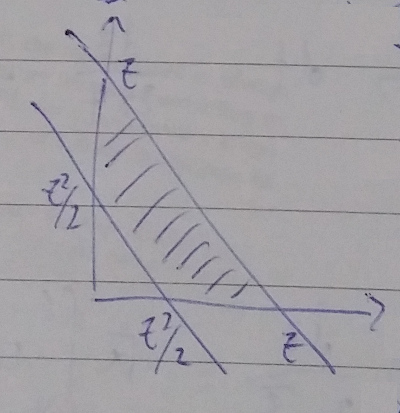
\includegraphics[scale=0.5]{q3b.jpg}
\end{center}

Volume is

\begin{align*}
  \int_0^2 \frac{z^2}{2} - \frac{z^4}{8} dz &= \frac{z^3}{6} - \frac{z^5}{40}\bigg]_0^2 \\
  &= \frac{8}{6} - \frac{32}{40} \\
  &= \frac{8 * 20 - 32 * 3}{120} \\
  &= \frac{64}{120} \\
  &= \frac{8}{15}
\end{align*}

\end{document}
